% vi:ft=tex
\documentclass[utf8,10pt]{beamer}

\usepackage[english]{babel}
\usepackage{etex}
\usepackage{pgf}
\usepackage[absolute,overlay]{textpos}
\usepackage{tikz}
\usepackage{listings}
\usepackage{graphicx}
\usepackage{pgfplots}
\usepackage{standalone}
\usepackage{enumitem}
%\usepackage[bitstream-charter]{mathdesign}
\usepackage{berasans}
\usepackage[backend=biber,style=alphabetic]{biblatex}
\usepackage{multirow}
\usepackage{mathtools}
\usepackage{ragged2e}
\usepackage{minted}
\usepackage{verbatim}
\usepackage{amssymb}
\usepackage{amsfonts}
\usepackage{textcomp}

\usetikzlibrary{arrows, shapes, positioning, trees,calc,intersections}
\mode<presentation>

% 45 degree rotated column descriptor
\usepackage{adjustbox}
\usepackage{array}

\usetheme[noheader,smallrightmargin,smallleftmargin,nosectionnum,heavyfont,pagenum]{tud}
\addbibresource{../Related_Work.bib}

\setbeamertemplate{footnote}
{
  %\scriptsize
  \tiny
  \noindent%
  \insertfootnotemark~\insertfootnotetext
}

\setbeamertemplate{enumerate items}[default]
\setbeamertemplate{itemize items}[triangle]

\title[]{Behaviour-Aware Load Balancing for a Micro-Kernel}

\author{Philipp Eppelt}

\date{04.03.2015}
\datecity{Dresden}

\einrichtung{Fakult\"a{}t Informatik}

\institut{Institut f\"u{}r Systemarchitektur}
\professur{Lehrstuhl f\"u{}r Betriebssysteme}


\begin{document}

\maketitle

\large

\newcommand{\ft}[1]{\frametitle{\hfill #1}}

% motivation
%%%%%%%%%%%%%%%%%%%%%%%%%%%%%%%%%%%%%%%%%%%%%%%%%%%%%%%%%%%%%%%%%%%%%%%%%%%%%%

\begin{frame}
  \frametitle{}
  \centering
  \includegraphics[width=\columnwidth]{../images/cpu_mem_gap}
\end{frame}


\begin{frame}
  \frametitle{}
  \centering
  \includegraphics[width=\columnwidth]{../images/mem_access_hierarchy_latency}
\end{frame}


% state of the art
%%%%%%%%%%%%%%%%%%%%%%%%%%%%%%%%%%%%%%%%%%%%%%%%%%%%%%%%%%%%%%%%%%%%%%%%%%%%%%
% service architecture
%%%%%%%%%%%%%%%%%%%%%%%%%%%%%%%%%%%%%%%%%%%%%%%%%%%%%%%%%%%%%%%%%%%%%%%%%%%%%%
\begin{frame}
  \frametitle{haswell cache architecture}
  \centering
  \begin{minipage}[l]{.49\columnwidth}
    \includestandalone[mode=tex,width=\columnwidth]{../images/haswell_core_layout}
  \end{minipage}
  \begin{minipage}[r]{.49\columnwidth}
    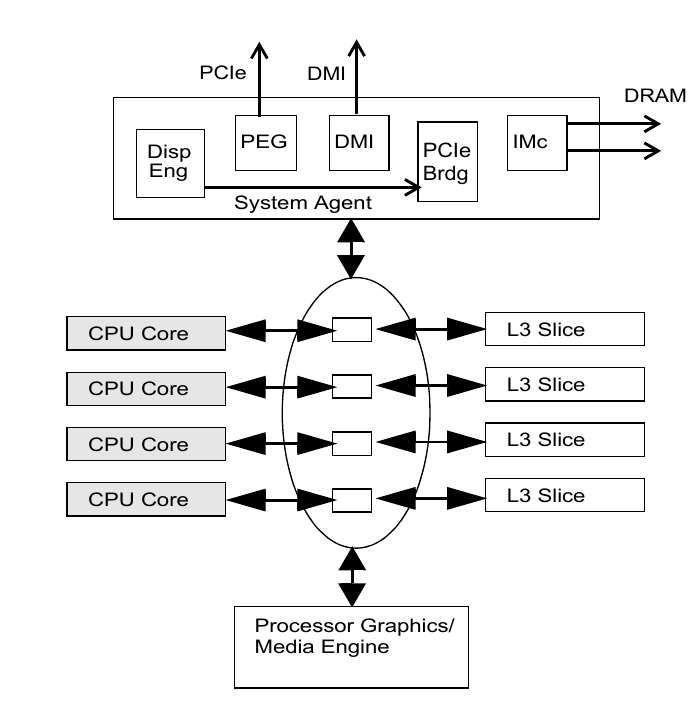
\includegraphics[scale=.27]{../images/haswell_architecture_by_intel_large_cropped}
  \end{minipage}
\end{frame}

\begin{frame}
  \frametitle{adjustment cycle executed each interval}
  \centering
  \includestandalone[mode=tex,width=.6\columnwidth]{../images/statusvortrag/arch_interval_cycle}
\end{frame}



\begin{frame}
  \frametitle{system layout}
  \centering
  \includestandalone[mode=tex,width=.7\columnwidth]{../images/system_layout_with_loadBalancer}
\end{frame}


\begin{frame}[fragile]
  \frametitle{}
  \centering
  \begin{minipage}[c]{\columnwidth}
    \begin{minted}[]{lua}
ld:start({  caps = { },
    scheduler = threadMapperFactory:create(
      L4.Proto.Scheduler,
      "min_prio = 0", "max_prio = 5",
      "distr=fract" ),
    log = { "client", "green" }
  },
  "rom/ex_fractal");
    \end{minted}
  \end{minipage}
\end{frame}


% future work 
%%%%%%%%%%%%%%%%%%%%%%%%%%%%%%%%%%%%%%%%%%%%%%%%%%%%%%%%%%%%%%%%%%%%%%%%%%%%%

\begin{frame}
  \frametitle{Future Work}
  \centering
  \begin{itemize}
    \item delayed measurement fix
    \item Intel CAT and CMT
    \item hierarchical load balancing
    \item multi-socket and distributed systems
    \item heterogeneous systems
  \end{itemize}
\end{frame}

\end{document}
